\bluepage{Přehled architektury GPU}

\begin{frame}
\frametitle{GPU architektura v průběhu let (AMD)}
	\begin{itemize}
	\item Nejprve pouze 2D akcelerace
	\item Poté 3D akcelerace, specializovaný HW
	\item Dál částečně programovatelná pipeline
	\item Nyní velké množství výpočetních jednotek pro obecné výpočty (2D akcelerace emulovaná pomocí 3D)
	\end{itemize}
	\begin{figure}[h]
	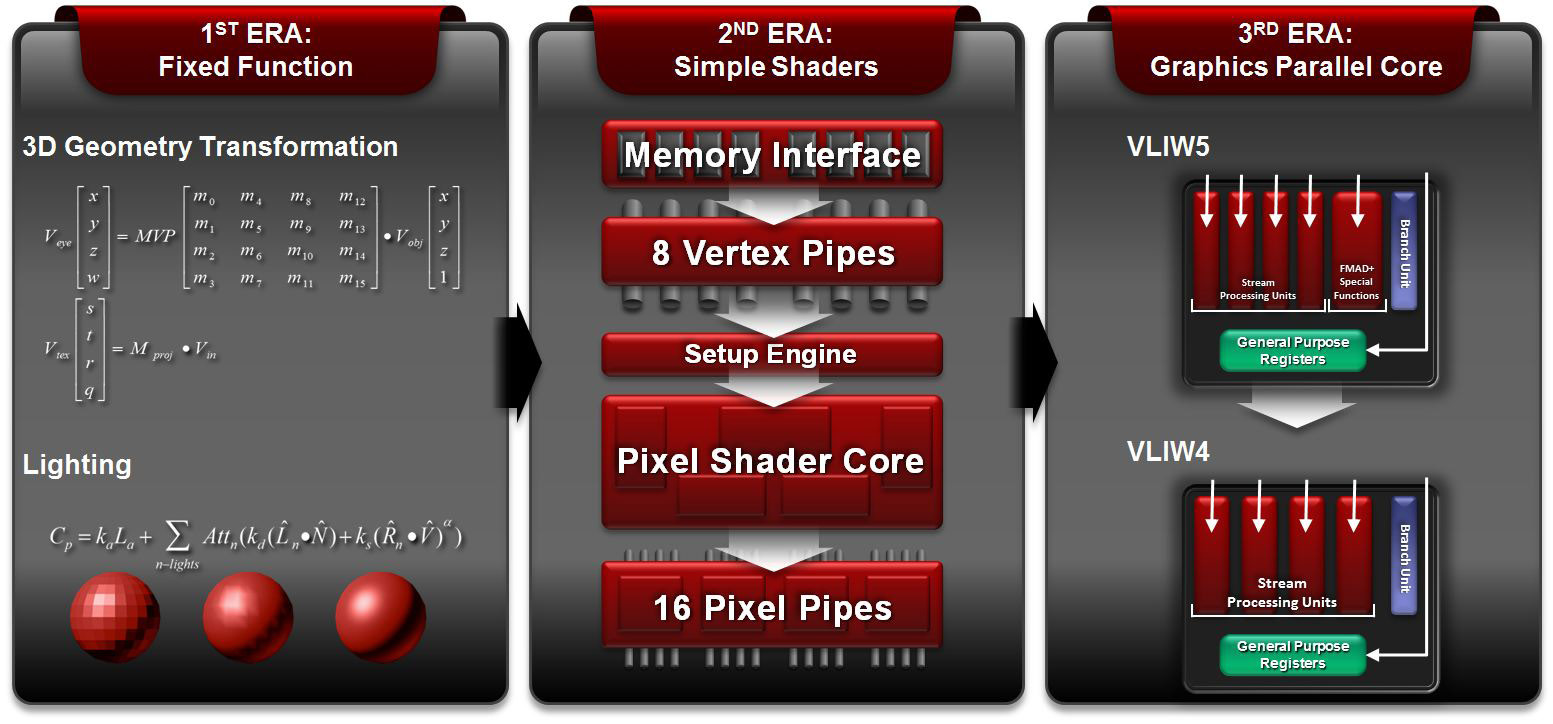
\includegraphics[width=10cm,keepaspectratio]{pics/gpu/gpu_amdevoluce}
	\end{figure}
\end{frame}

\begin{frame}
\frametitle{GPU vs CPU}
	\begin{itemize}
	\item CPU - málo, velmi výkonných výpočetních jednotek
	\item Velká keš, velké řízení, vykonávání instrukcí mimo pořadí, ...
	\item GPU - velké množství méně výkonných, jednodušších výpočetních jednotek
	\item Malé keše, malé řízení, víc tranzistorů pro výpočty, ...
  \item GPU - data parallel, náznak task parallel
  \item CPU - tast parallel
	\end{itemize}
	\begin{figure}[h]
	
\includegraphics[width=10cm,keepaspectratio]{pics/gpu/gpu_gpuvscpu.pdf}
	\end{figure}
\end{frame}

\begin{frame}
\frametitle{GPU vs CPU}
	\begin{figure}[h]
	
\includegraphics[width=10cm,keepaspectratio]{pics/gpu/gpu_common}
	\end{figure}
	\begin{itemize}
	\item Grafická karta je složena z několika multiprocesorů a grafické paměti.
  \item Nvidia - streaming multi processor (SM).
  \item AMD   - compute unit (CU).
  \item Tento multiprocessor je dále složen z velkého množství jader a různých druhů pamětí.
  \item Akce, která beží na jednom multiprocesoru je nezávislá na akci, která běží na jiném multiprocesoru.
  \item Jádra bývají označována jako shader unit (AMD Radeon HD7970M 20xCU, 64 shader unit na CU, = 1280 shader unit).
	\end{itemize}
\end{frame}

\begin{frame}
\frametitle{NVIDIA - GTX 1080}
	\begin{figure}[h]
	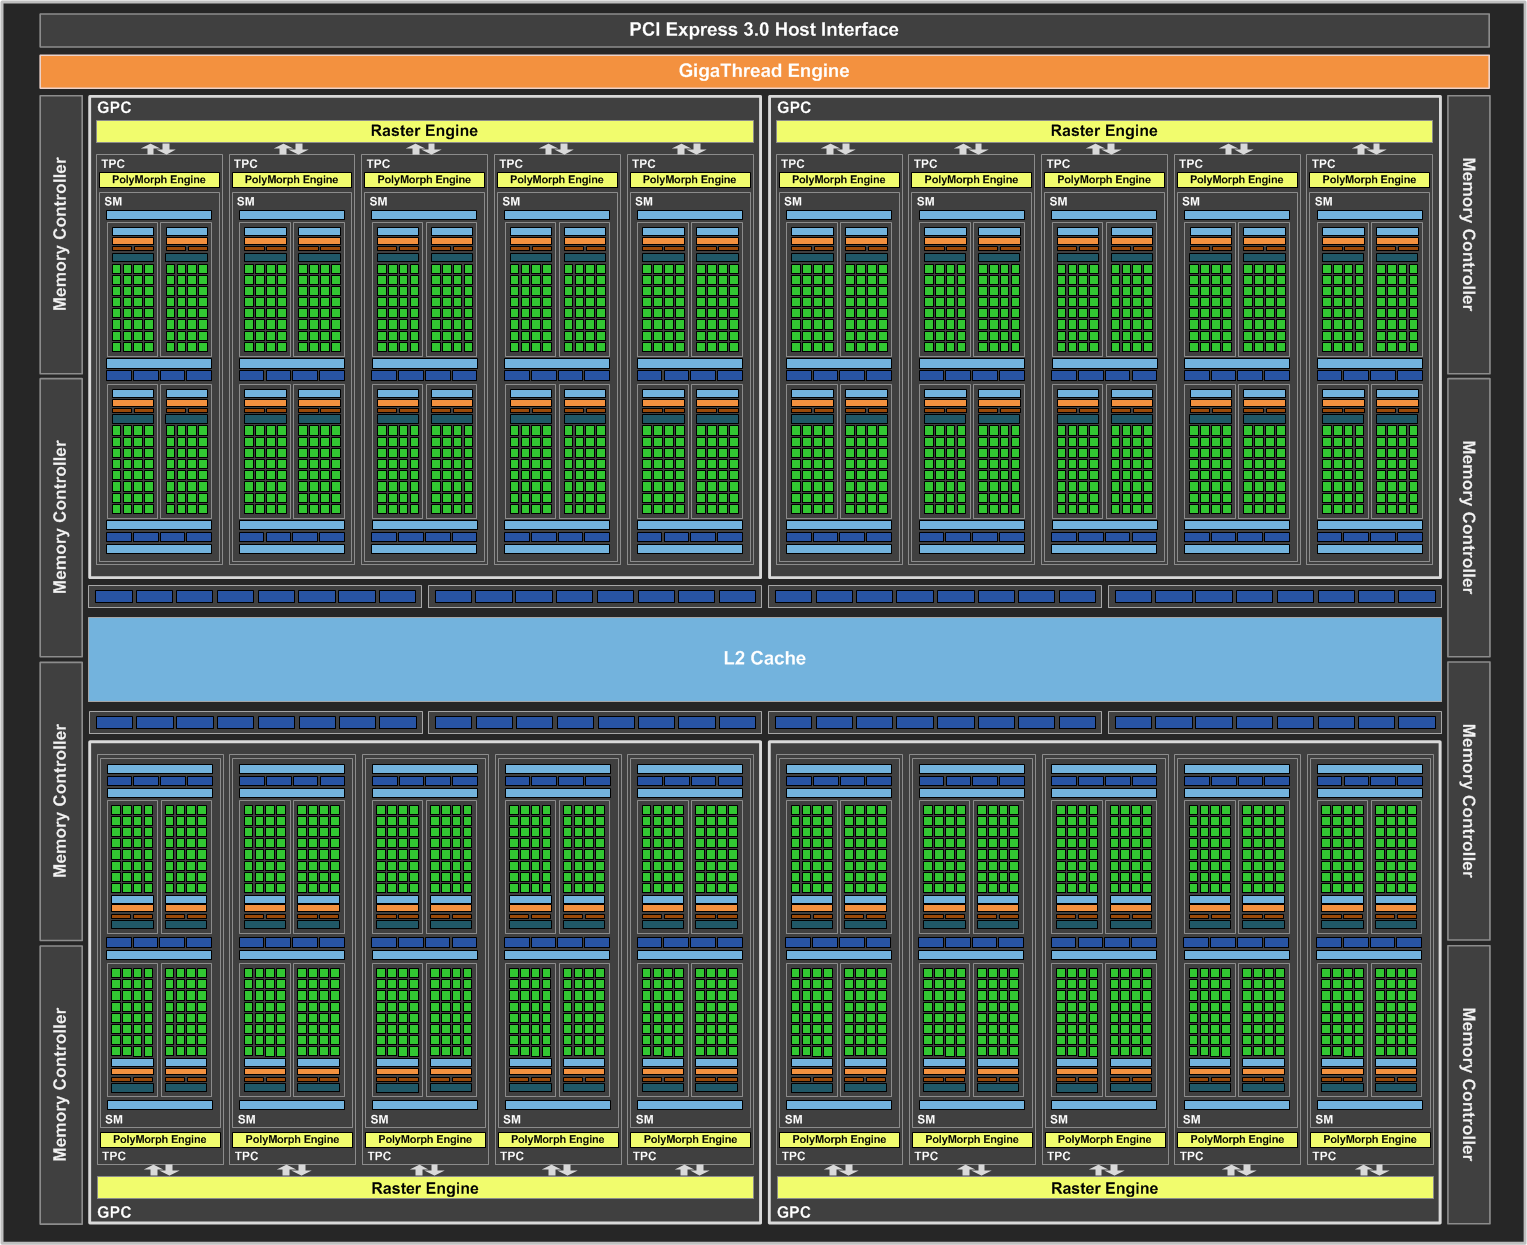
\includegraphics[width=8.5cm,keepaspectratio]{pics/gpu/1080}
	\end{figure}
\end{frame}

\begin{frame}
\frametitle{AMD FuryX/fiji}
	\begin{figure}[h]
	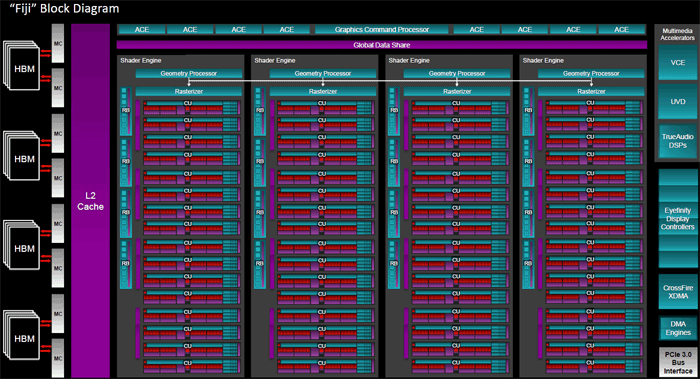
\includegraphics[width=11cm,keepaspectratio]{pics/gpu/furyx}
	\end{figure}
\end{frame}

\begin{frame}
\frametitle{NVIDIA - Fermi SMX}
	\begin{figure}[h]
	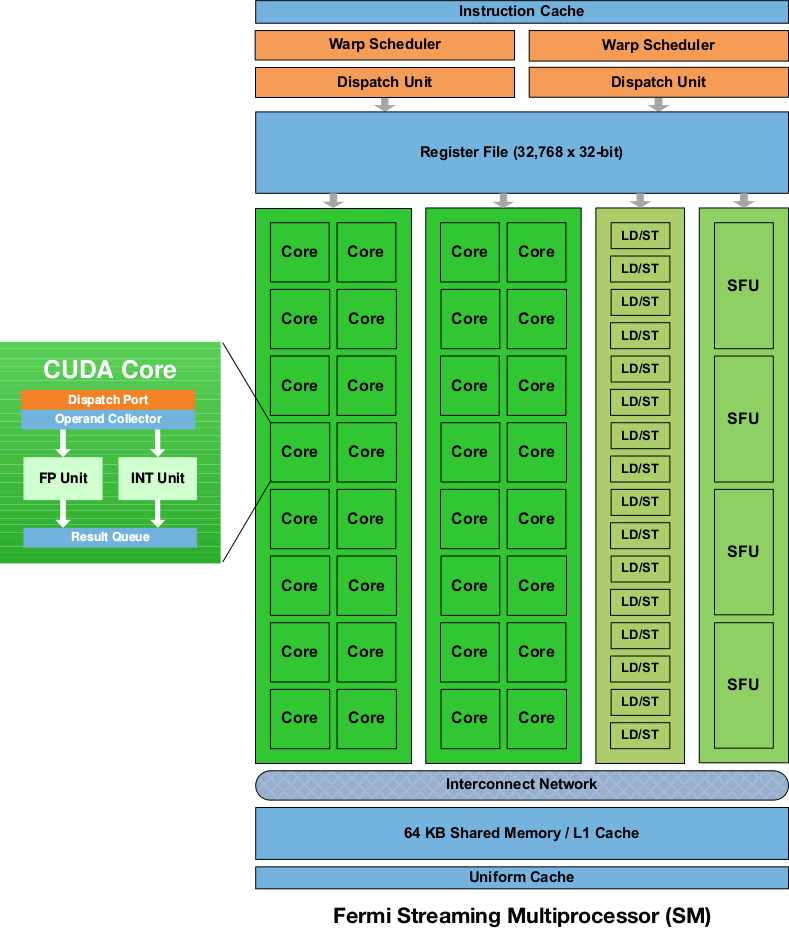
\includegraphics[width=7cm,keepaspectratio]{pics/gpu/fermi}
	\end{figure}
\end{frame}

\begin{frame}
\frametitle{NVIDIA - 1080 SMX}
	\begin{figure}[h]
	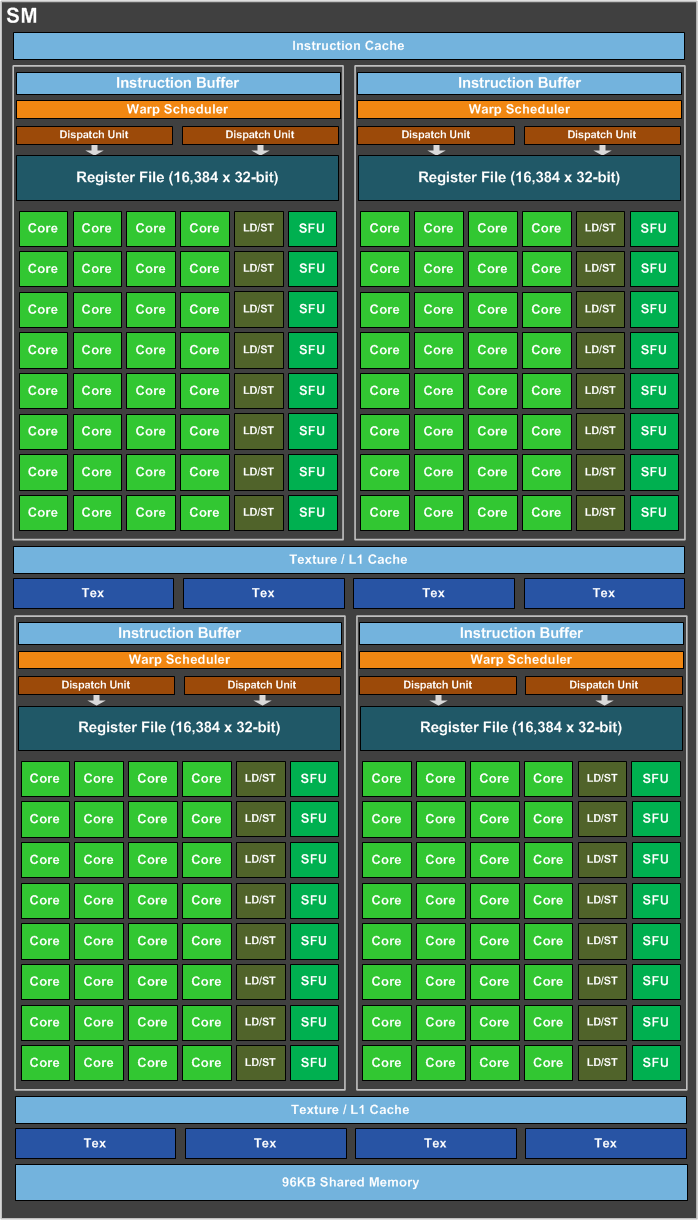
\includegraphics[width=4.5cm,keepaspectratio]{pics/gpu/1080SMX}
	\end{figure}
\end{frame}

\begin{frame}
\frametitle{AMD - GCN}
	\begin{figure}[h]
	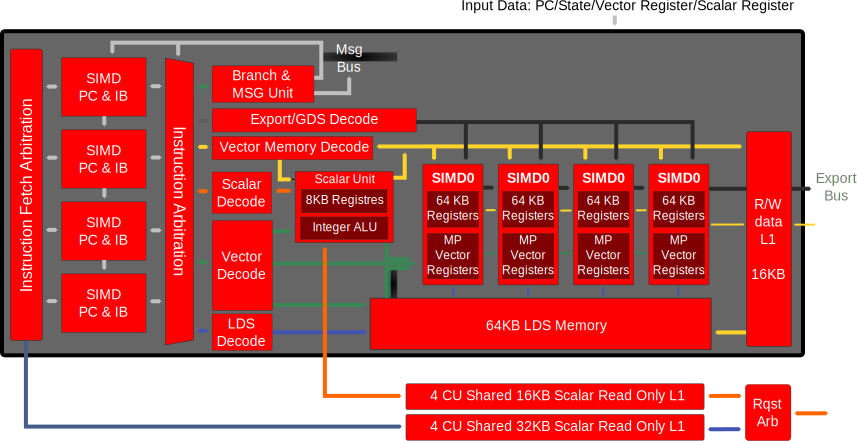
\includegraphics[width=11cm,keepaspectratio]{pics/gpu/gcn}
	\end{figure}
\end{frame}

\begin{frame}
\frametitle{Hardwarové části}
	\begin{itemize}
	\item Dnešní GPU jsou značně programovatelné
  \item Některé části stále zůstávají hardwarově zadrátované
  \item Rasterizace - převod trojúhelníků na fragmenty
  \item Tessellace - rozřezání polygonů na mnoho podpolygonů
  \item Texturovací jednoty - filtrování, opakování na okrajích, ...
  \item Depth buffer, Stencil buffer, ...
  \item A další
  \item Ke většině lze přistoupit pouze z některých API (OpenGL, Vulkan, DirectX)
	\end{itemize}
\end{frame}

\begin{frame}
  \frametitle{Paměťová hierarchie}
  \begin{columns}[T]
    \begin{column}{.48\textwidth}
      \begin{figure}[h]
        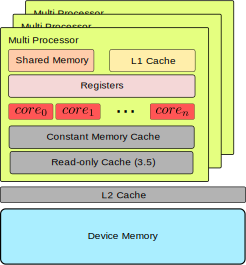
\includegraphics[width=5cm,keepaspectratio]{pics/gpu/memory_hierarchy}
      \end{figure}
    \end{column}
    \begin{column}{.48\textwidth}
      \begin{itemize}
        \item Spousta různých pamětí s různou velikostí a rychlostí.
        \item Obecně platí, čím blíže k jádru, tím rychlejší a tím menší.
        \item Registry jsou nejrychlejší (na Kepleru jich je 65536 x 32bit).
        \item Sdílená paměť slouží pro komunikaci mezi vlákny.
        \item Device memory (global memory) je velká (2GB i více), ale pomalá paměť.
      \end{itemize}
    \end{column}
  \end{columns}
\end{frame}

\begin{frame}
  \frametitle{Vláknová hierarchie}
  \begin{itemize}
    \item Na GPU pouštíme instance kernelů - vlákna.
    \item Kernel je program složený z instrukcí (podobně jako shader) a běží ve vláknu.
    \item Instrukce v kernelu jsou spouštěny v mnoha instancích na jádrech SM.
    \item Vlákna (thread, invocation, work-item) jsou seskupovány do pracovních skupin (work-group).
    \item Vlákna v pracovních skupinách můžou být na sobě závislá.
    \item Skupiny můžou být 1D, 2D, 3D (určuje pořadí vláken a jejich index).
    \item Mnoho work-group tvoří dispatch (taky může být 1D, 2D, 3D).
    \item Terminologie se liší (OpenCL, Cuda, Compute Shader, ...).
  \end{itemize}
\end{frame}

\begin{frame}
  \frametitle{Vláknová hierarchie - Compute shadery}
  \begin{picture}(320,250)
		\put(-28,50){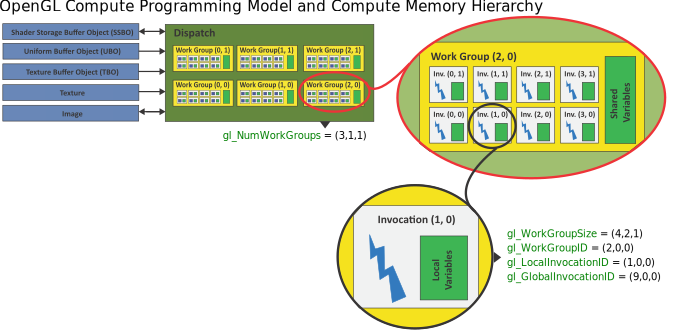
\includegraphics[height=6.4cm]{pics/gpu/threadHierarchy}}
	\end{picture}
\end{frame}

\begin{frame}
  \frametitle{Vláknová hierarchie}
  \begin{figure}[h]
	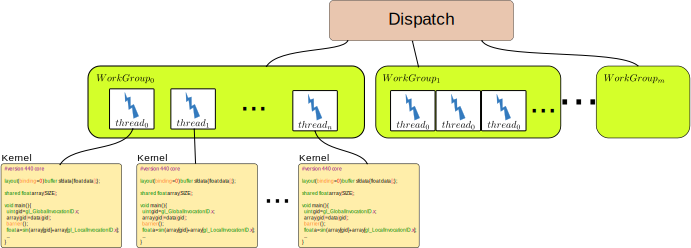
\includegraphics[width=11cm,keepaspectratio]{pics/gpu/thread_hierarchy}
	\end{figure}
  \begin{itemize}
    \item Vlákna jsou seskupena do skupin work-group.
    \item Work-group může být 1D, 2D, 3D.
    \item Work-groupy jsou seskupeny do dispatch.
    \item Dispatch může být také 1D, 2D, 3D.
    \item Na jeden SM se může pustit vícero Work-group, pokud na to vystačí zdroje (registry, sdílená paměť)!
  \end{itemize}
\end{frame}

